\section{Lidar detection range analysis}
It is useful to know possible range of detection based on lidar sensor. This range influences the way how the waypoints for exploration are generated. Higher the detection range is, lower number of waypoints is necessary for exploring whole arena. There is a limited time for exploration, because brick pickup and brick placement takes a lot of time. Speed of pickup and placement is limited mainly by the speed of Kinova arm. We estimate the maximal range using the figure \ref{fig:range}.

\begin{figure}[H]
\centering
\includegraphics[scale=1.1]{fig/lidar_range.png}
\caption[Lidar range study]{Visualization of rays hitting the red brick.}
\label{fig:range}
\end{figure}

Angle $\alpha$ is the resolution of lidar known from table \ref{tab:lidar}. Only the maximal range is calculated thus angle $\beta = 90\degree$. To obtain the distance between points on the brick the cosine theorem can be used.
\begin{equation}
a^2 = b^2 + c^2 - 2bc \cos \alpha.
\end{equation}
Because $\beta$ is right angle we can write $b = c$ and thus:
\begin{equation}
a = \sqrt{2b^2 \left(1-\cos \alpha \right)}.
\end{equation}
Now we want to know how many rays $N$ would hit the brick from given distance $b$ with lidar angular resolution $\alpha$ and size of the brick $a$. 
\begin{align}
a &= \sqrt{2b^2 \left(1-\cos \left( N \alpha \right) \right)} \\
N &= \frac{\arccos\left(1-\frac{a^2}{2b^2}\right) }{\alpha}
\label{eq:rays}
\end{align}
Finally we can plot a function of number of rays $N$ with respect to distance to object $b$. This analysis can be done similarly for vertical and horizontal resolution.

\begin{figure}[H]
\centering
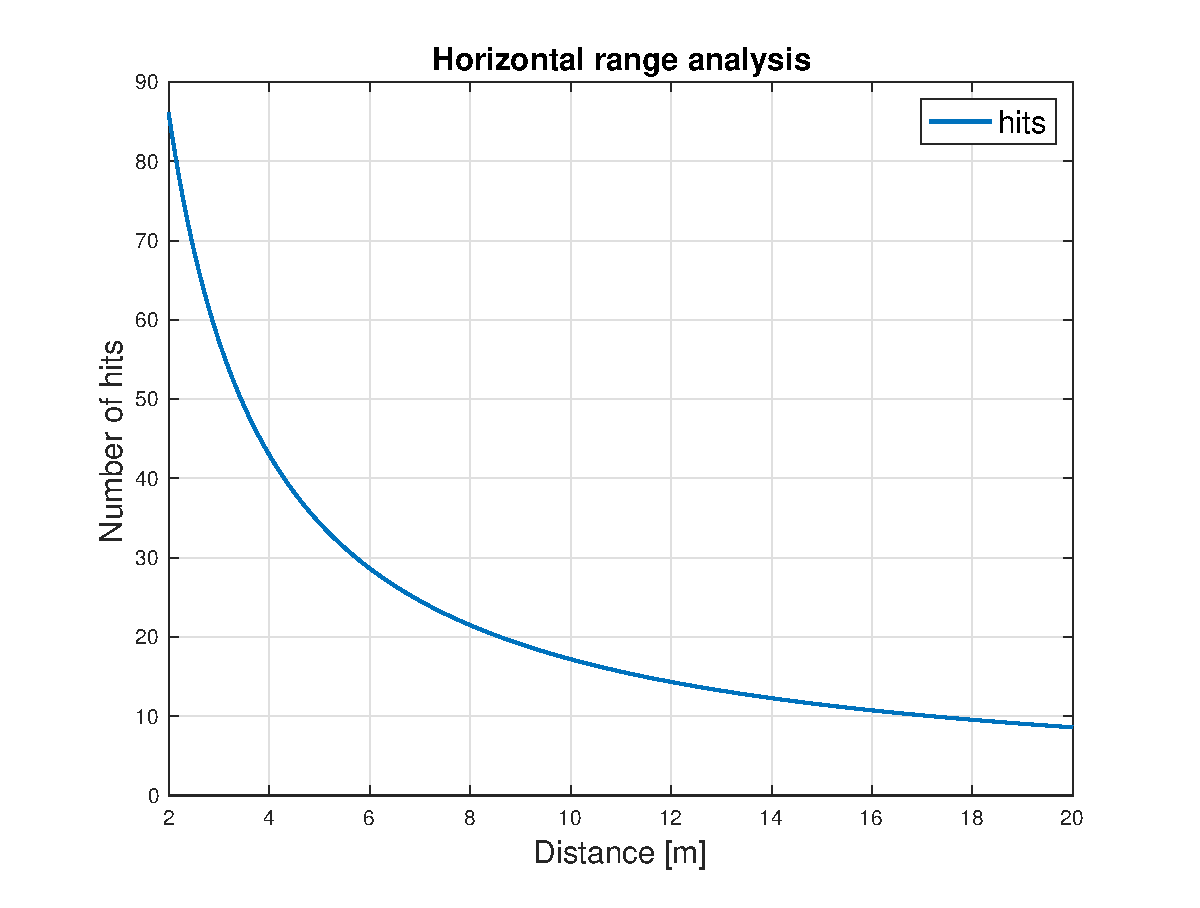
\includegraphics[scale=0.5]{fig/horizontal_range.eps}
\caption[Horizontal range chart]{Number of hits of the smallest brick from given distance.}
\label{fig:horizontal_hits}
\end{figure}

In the figure \ref{fig:horizontal_hits} is clearly visible that the horizontal resolution of the lidar is not limiting factor of the range. Even from 10 meters is lidar able to hit red brick more than 15 times. On the other hand the figure \ref{fig:vertical_hits} shows that pile of bricks with height 40 cm would be hit by less than two lidar layers from distance bigger than 6 meters. Furthermore this is the best case scenario analysis where $\beta$ is right angle which happens rarely in reality.
 
\begin{figure}[H]
\centering
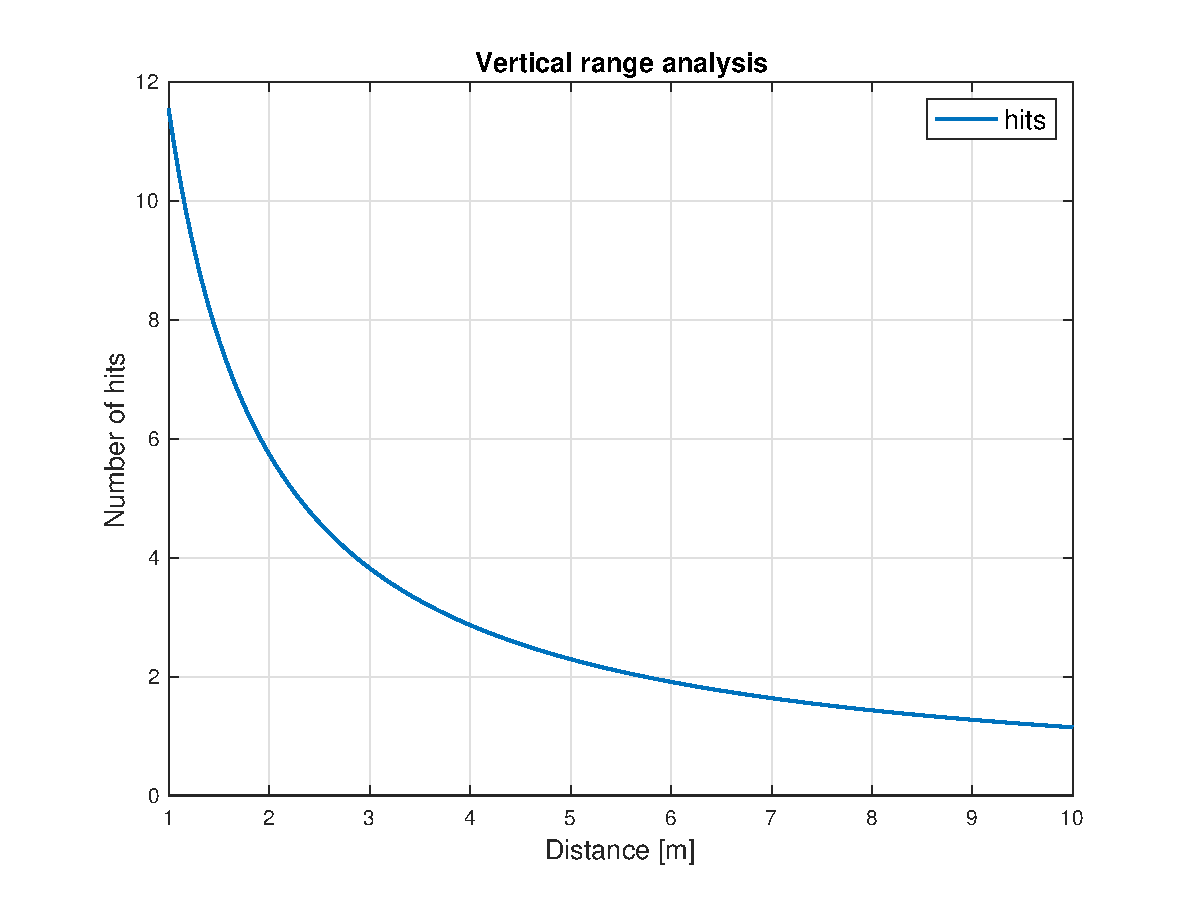
\includegraphics[scale=0.5]{fig/vertical_range.eps}
\caption[Horizontal range chart]{Number of hits of two stacked bricks from given distance.}
\label{fig:vertical_hits}
\end{figure}


\section{Detection pipeline}
Detection is divided into three parts. All three parts are discussed in next three subsections. detection pipeline is visualized in the figure \ref{fig:flowchart}. 

\hspace{5px}
\begin{figure}[H]
\centering
\includegraphics[scale=0.06]{fig/flowchart.pdf}
\caption[Program pipeline]{Visualization of subsequent steps of detection.}
\label{fig:flowchart}
\end{figure}

It can be seen that the symbolic map has two types of inputs. The main advantage of this approach is that it extends the lidar detection range. As we discussed in previous section, used lidar has low vertical resolution - only 16 layers. Thus the bricks are often visible in only one layer of lidar scan. If we use only one scan, there is a high probability of false positive measurements. On the one hand we can decrease the occurrence of false positives by adding other lidar layers into the detection process. But on the other hand two layers are available only from distance smaller than 6 meters and that decreases the detection range. Therefore we exploited both approaches. One layer line segmentation for generating the candidates with low confidence and multilayer pile detector providing high quality estimates.

\subsection{Line segmentation}
For line segmentation is used IEPF algorithm very similar to the one described in algorithm \ref{alg:segmentation}. Only the final merging parallel segments is omitted, because it can connect two bricks into one. After retrieving the segments, a filtering based on the segment size is done. It is possible to assign the color to the segment because each brick type has unique dimensions. Example of lidar measurement with extracted and filtered lines is in the figure \ref{fig:segments}. Algorithm performance is influenced by correct setup of constants $C$ and $S$ (clustering and splitting distance). If we choose to high C, it could happen that the algorithm joins two bricks into one segment. As described in figure \ref{fig:piledef} the distance between two bricks of same color is 10 cm. Therefore the clustering distance must be always less than 10 cm. If the clustering distance is too low, one brick can be unintentionally divided into many segments and without merging at the end are these segments useless. It is necessary to bear in mind that the lidar precision as shown in table \ref{tab:lidar} is $\pm3$ cm so any clustering with distance smaller than 6 cm will be highly affected be sensor noise. Found segments are transformed into the map frame and passed to symbolic map as low confidence detections. Further are segments passed to pile detector which can filter out false positive detections.

\hspace{8mm}

\begin{figure}[H]
\centering
\includegraphics[scale=0.43]{fig/segments}
\caption[Line segmentation visualization]{RViz visualization of line segmentation. In the figure is evident that the bricks are well detected. This detection is done from $\approx3$m. There is visible one false positive detection behind the brick piles on the tree.}
\label{fig:segments}
\end{figure}


\subsection{Pile detection}

\subsection{Pattern fitting}
